% -- Document configuration
\documentclass{article}

% -- Input and language settings
% \usepackage[utf8]{inputenc}
\usepackage[spanish]{babel}
\decimalpoint                             % From babel package to use points instead of commas in decimals

% -- Page and line settings
\usepackage{geometry}
\geometry{letterpaper, 
    % margin=2cm, 
    left=3cm, right=3cm,
    top=1.2cm, bottom=1.2cm,
    includefoot, 
    includehead}
\renewcommand{\baselinestretch}{1.2}

% -- Required packages
\usepackage{xcolor}
\usepackage[many]{tcolorbox}
\usepackage{mathtools,amsfonts,amsmath}     % Loads amsmath if not already loaded
\allowdisplaybreaks                         % To allow page breaks if equations are too long
\usepackage[parfill]{parskip}               % No indent and separation lines for paragraphs
\usepackage{cancel}                         % To cancel math terms
\usepackage[shortlabels]{enumitem}          % To handle enumerations
\usepackage{tikz}
\usetikzlibrary{automata, arrows.meta, positioning}
\usepackage[mode=buildnew]{standalone}      % To import figures in standalone files
\usepackage[hidelinks]{hyperref}
\usepackage[spanish]{cleveref}              % To use autocompleted reference labels, language must be change as in babel package
\usepackage{caption}                        % Caption and subcaption to allow subfigures
\usepackage{subcaption}
\usepackage{float}                          % To specify the location of figures
\usepackage{multicol}                       % To use multicolumns
\usepackage[bottom]{footmisc}               % To locate footnotes at the bottom

% -- Title and heading settings
\usepackage{titling}
\usepackage{fancyhdr}
\pagestyle{fancy}

% -- Code and code formatting
\usepackage{minted}                         % To insert code
\usemintedstyle[julia]{gruvbox-light}       % Code theme and language
\definecolor{bg}{rgb}{0.98, 0.97, 0.88}     % Code block background

\usepackage{fontspec}                       % To allow the use of monospace fonts
\setmonofont{JuliaMono}[Path=./codefonts/, Extension=.ttf, UprightFont=*-Regular, ItalicFont=*-RegularItalic, Scale=0.75]

\usepackage{fancyvrb}                       % To change line number font
\renewcommand{\theFancyVerbLine}{\textcolor{gray}{\footnotesize\texttt{\arabic{FancyVerbLine}}}}

\definecolor{light-gray}{gray}{0.95}        % Color, box and style to show small code thingys inside normal text
\newcommand{\code}[1]{\colorbox{light-gray}{\texttt{#1}}}

% -- Bilbiography preferences
\usepackage[square,numbers]{natbib}
\bibliographystyle{unsrt}

% -- Footnotes without numbering
\newcommand\nnfootnote[1]{%
  \begin{NoHyper}
  \renewcommand\thefootnote{}\footnote{#1}%
  \addtocounter{footnote}{-1}%
  \end{NoHyper}
}

% -- Theorems
\newtheorem{theorem}{Theorem}

\lhead{\theinstitution\ -- \thedepartment}
\chead{}
\rhead{Programación para la IA\ -- \thetitle}
\lfoot{}
\cfoot{\thepage}
\rfoot{}

% -- Problem solution
\newenvironment{solution}
{\begin{quote}
\textbf{Solución:}\medskip

}
{

\hfill\rule{0.5\textwidth}{0.5pt}
\end{quote}}

% -- Equation result
\newcommand{\result}[1]
{
\tcbhighmath[colframe=white, colback=gray!15, sharp corners]
{#1}
}

% -- Function definitions
\newcommand{\dprod}[2]{{#1} \cdot {#2}}
\newcommand{\txtgray}[1]{\textcolor{gray}{#1}}

% -- Author information
\title{Actividad 5}
\author{Leonardo Flores Torres}
\newcommand\theinstitution{Universidad Veracruzana}
\newcommand\thedepartment{Inteligencia Artificial}
\newcommand\thecourse{Programación para la Inteligencia Artificial}

% -- Paths
% \newcommand\codelists{../programs/lists.rkt}

% Remove red color boxes of "syntax errors" in minted
\AtBeginEnvironment{minted}{%
  \renewcommand{\fcolorbox}[4][]{#4}}

% -- Document
\begin{document}

\thispagestyle{empty}

%Title
\begin{center}
\textsc{\theinstitution}\\[2mm]

\thedepartment

\rule{0.6\textwidth}{0.5pt}\\[2mm]

\thecourse \\[4mm]

{\Large \textbf{\thetitle}}\\[2mm]

\theauthor \\[2mm]

{\small \today}
\end{center}
\medskip

% -- 
\vspace{1cm}

Reunir un conjunto de 15 documentos de 5 clases. Cada documento de al menos 1 página. Seleccionar 10 documentos de cada clase aleatoriamente para realizar el entrenamiento bajo el esquema de bolsa de palabras.
\begin{itemize}
    \item Emplear los 5 documentos restantes de clada clase para clasificar empleando el teorema de Bayes.
    \item Resumir sus resultados empleando una matriz de confusión.
    \item Calcular métricas TP, TN, FP, FN por clase, y tambiém calcular Accuracy, Precision, Recall, Specificity, y F1-Score por clase.
    \item Discutir los resultados obtenidos.
\end{itemize}

Todos los libros usados para este trabajo fueron obtenidos de la plataforma gratuita de libros Project Gutenberg\footnote{\url{https://www.gutenberg.org/}}, en la cual los libros estan clasificados por categorías las cuales fueron usadas como los nombres de los directorios en donde se almacenaron los libros. A continuación se muestra un listado de los libros usados para el conjunto de entrenamiento guardados en el directorio \code{training-dataset}:
\begin{minted}[
    frame=none,
    % autogobble,
    obeytabs=false,
    breaklines,
    tabsize=4,
    linenos=false,
    baselinestretch=1,
    firstnumber=1,
    bgcolor=bg!70,
    ]{bash}
    ❯ exa --tree -L=2 train-dataset/
    training-dataset
    ├── biology
    │  ├── an-elementary-study-of-insects.txt
    │  ├── concerning-animals-and-other-matters.txt
    │  ├── contributions-to-the-theory-of-natural-selection.txt
    │  ├── life-history-of-the-kangaroo-rat.txt
    │  ├── the-origin-of-species.txt
    │  └── the-story-of-the-living-machine.txt
    ├── chemistry
    │  ├── elements-of-chemistry.txt
    │  ├── on-laboratory-arts.txt
    │  ├── on-the-antiquity-of-the-chemical-art.txt
    │  ├── the-chemical-history-of-a-candle.txt
    │  ├── the-history-of-phosphorus.txt
    │  └── the-story-of-alchemy-and-the-beginnings-of-chemistry.txt
    ├── fiction
    │  ├── a-little-journey.txt
    │  ├── alices-adventures-in-wonderland.txt
    │  ├── around-the-world-in-eighty-days.txt
    │  ├── in-the-year-2889.txt
    │  ├── the-adventures-of-sherlock-holmes.txt
    │  ├── the-great-gatsby.txt
    │  ├── the-scarlet-letter.txt
    │  └── the-world-set-free.txt
    ├── horror
    │  ├── dracula.txt
    │  ├── metamorphosis.txt
    │  ├── scotish-ghost-stories.txt
    │  ├── the-call-of-cthulhu.txt
    │  ├── the-dunchich-horror.txt
    │  ├── the-legend-of-sleepy-hollow.txt
    │  └── the-mysteries-of-udolpho.txt
    ├── music
    │  ├── contemporary-american-composers.txt
    │  ├── essentials-in-conducting.txt
    │  ├── for-every-music-lover.txt
    │  ├── how-to-sing.txt
    │  └── life-of-chopin.txt
    ├── poetry
    │  ├── men-and-women.txt
    │  ├── poems-by-walt-whitman.txt
    │  ├── the-new-morning-poems.txt
    │  ├── the-rime-of-the-ancient-mariner.txt
    │  ├── the-waste-land.txt
    │  ├── the-works-of-horace.txt
    │  ├── underwoods.txt
    │  └── violets-and-other-tales.txt
    └── politics
       ├── a-preface-to-politics.txt
       ├── anarchism-and-other-essays.txt
       ├── political-ideals.txt
       ├── the-communist-manifesto.txt
       └── utopia.txt
\end{minted}

La selección aleatoria de libros fue confusa de implementar, en vez de eso se descargaron más libros pertenecientes a las mismas categorías de los mostrados anteriormente guardados en una carpeta llamada \code{test-dataset}:
\begin{minted}[
    frame=none,
    % autogobble,
    obeytabs=false,
    breaklines,
    tabsize=4,
    linenos=false,
    baselinestretch=1,
    firstnumber=1,
    bgcolor=bg!70,
    ]{bash}
    ❯ exa --tree -L=2 test-dataset/
    test-dataset
    ├── biology
    │  ├── evolution-old-and-new.txt
    │  └── the-dancing-mouse.txt
    ├── chemistry
    │  ├── an-elementary-study-of-chemistry.txt
    │  └── the-sceotical-chymist.txt
    ├── fiction
    │  └── the-lost-king-of-oz.txt
    ├── horror
    │  ├── the-great-god-pan.txt
    │  └── the-wendigo.txt
    ├── music
    │  └── musical-memories.txt
    ├── poetry
    │  ├── poems-of-sidney-lanier.txt
    │  └── the-complete-poems-of-sir-thomas-moore.txt
    └── politics
       ├── leviathan.txt
       └── the-prince.txt
\end{minted}

Del resultado de la terminal se puede observar que las categorías elegidas fueron las siguientes
\begin{itemize}
    \item \code{\quotes{chemistry}},
    \item \code{\quotes{poetry}},
    \item \code{\quotes{fiction}},
    \item \code{\quotes{biology}},
    \item \code{\quotes{horror}},
    \item \code{\quotes{music}},
    \item \code{\quotes{politics}}.
\end{itemize}

Este trabajo fue realizado usando el lenguaje de programación \code{python}. Este contiene ya muchas librerías con las funcionalidades que se podrían llegar a necesitar para cumplir con los puntos requeridos. Primero se cargan las librerias necesarias:
\begin{minted}[
    frame=none,
    autogobble,
    obeytabs=false,
    breaklines,
    tabsize=4,
    linenos=true,
    baselinestretch=1,
    firstnumber=1,
    bgcolor=bg!70,
    ]{python}
    import pathlib    # To handle files
    import numpy as np    # To handle arrays as numpy arrays
    import matplotlib.pyplot as plt    # For plotting purposes

    from sklearn.feature_extraction.text import CountVectorizer
    from sklearn.model_selection import train_test_split
    from sklearn.naive_bayes import MultinomialNB
    from sklearn.metrics import accuracy_score
    from sklearn.metrics import confusion_matrix
    from sklearn.metrics import classification_report
\end{minted}

Posteriormente se deben definir los directorios en donde se encuentran los conjuntos de entrenamiento y de prueba, respectivamente:
\begin{minted}[
    frame=none,
    autogobble,
    obeytabs=false,
    breaklines,
    tabsize=4,
    linenos=true,
    baselinestretch=1,
    firstnumber=11,
    bgcolor=bg!70,
    ]{python}
    working_dir = pathlib.Path().absolute()
    train_dir = working_dir / "training-dataset/"
    test_dir = working_dir / "test-dataset/"
\end{minted}

Para encontrar las categorías presentes en estos directorios se escribió la siguiente función:
\begin{minted}[
    frame=none,
    autogobble,
    obeytabs=false,
    breaklines,
    tabsize=4,
    linenos=true,
    baselinestretch=1,
    firstnumber=14,
    bgcolor=bg!70,
    ]{python}
    def get_categories_paths(files_dir):
        paths = []
        for item in files_dir.iterdir():
            if item.is_dir():
                paths.append(item)
        
        return paths
\end{minted}

En realidad no se obtienen las categorías sino el \code{path} de los directorios con cuyos nombres corresponden a las categorías, por ejemplo:
\begin{minted}[
    frame=none,
    autogobble,
    obeytabs=false,
    breaklines,
    tabsize=4,
    linenos=true,
    baselinestretch=1,
    firstnumber=1,
    bgcolor=\bgrepl,
    numberblanklines=false,
    ]{python}
    # REPL

    >>> categories_paths = get_categories_paths(train_dir)
    >>> categories_paths
    [PosixPath('/home/leo/Documents/mia/mia-activities/mia-2022-half2/mp/mp-proyecto/training-dataset/chemistry'),
    PosixPath('/home/leo/Documents/mia/mia-activities/mia-2022-half2/mp/mp-proyecto/training-dataset/poetry'),
    PosixPath('/home/leo/Documents/mia/mia-activities/mia-2022-half2/mp/mp-proyecto/training-dataset/fiction'),
    PosixPath('/home/leo/Documents/mia/mia-activities/mia-2022-half2/mp/mp-proyecto/training-dataset/biology'),
    PosixPath('/home/leo/Documents/mia/mia-activities/mia-2022-half2/mp/mp-proyecto/training-dataset/horror'),
    PosixPath('/home/leo/Documents/mia/mia-activities/mia-2022-half2/mp/mp-proyecto/training-dataset/music'),
    PosixPath('/home/leo/Documents/mia/mia-activities/mia-2022-half2/mp/mp-proyecto/training-dataset/politics')]
 \end{minted}

Posteriormente, de estos \code{path}s se extraen los últimos elementos de cada cadena para convertirlos en diccionarios y poder acceder a ellos de acuerdo a una palabra clave la cual, si es usada con el diccionario, 
\begin{minted}[
    frame=none,
    autogobble,
    obeytabs=false,
    breaklines,
    tabsize=4,
    linenos=true,
    baselinestretch=1,
    firstnumber=21,
    bgcolor=bg!70,
    ]{python}
    def get_categories(files_dir):
        categories_paths = get_categories_paths(files_dir)
        categories = dict()
        for path in categories_paths:
            category = path.as_posix().split("/")[-1]
            categories[category] = path
            
        return categories
\end{minted}

El siguiente ejemplo es una llamada a la función \code{get\_categories} con el \code{path} del conjunto de entrenamiento:
\begin{minted}[
    frame=none,
    autogobble,
    obeytabs=false,
    breaklines,
    tabsize=4,
    linenos=true,
    baselinestretch=1,
    firstnumber=1,
    bgcolor=\bgrepl,
    numberblanklines=false,
    ]{python}
    # REPL

    >>> categories = get_categories(train_dir)
    >>> categories
    {'chemistry': PosixPath('/home/leo/Documents/mia/mia-activities/mia-2022-half2/mp/mp-proyecto/training-dataset/chemistry'),
    'poetry': PosixPath('/home/leo/Documents/mia/mia-activities/mia-2022-half2/mp/mp-proyecto/training-dataset/poetry'),
    'fiction': PosixPath('/home/leo/Documents/mia/mia-activities/mia-2022-half2/mp/mp-proyecto/training-dataset/fiction'),
    'biology': PosixPath('/home/leo/Documents/mia/mia-activities/mia-2022-half2/mp/mp-proyecto/training-dataset/biology'),
    'horror': PosixPath('/home/leo/Documents/mia/mia-activities/mia-2022-half2/mp/mp-proyecto/training-dataset/horror'),
    'music': PosixPath('/home/leo/Documents/mia/mia-activities/mia-2022-half2/mp/mp-proyecto/training-dataset/music'),
    'politics': PosixPath('/home/leo/Documents/mia/mia-activities/mia-2022-half2/mp/mp-proyecto/training-dataset/politics')}
    
    >>> categories["horror"]
    PosixPath('/home/leo/Documents/mia/mia-activities/mia-2022-half2/mp/mp-proyecto/training-dataset/horror')
\end{minted}

Todavía es necesario listar de alguna manera los libros presentes por categoría, lo que es lo mismo, listar los archivos dentro de uno de los directorios de las categorías indicadas anteriormente:
\begin{minted}[
    frame=none,
    autogobble,
    obeytabs=false,
    breaklines,
    tabsize=4,
    linenos=true,
    baselinestretch=1,
    firstnumber=29,
    bgcolor=bg!70,
    numberblanklines=false,
    ]{python}
    def get_books_in_category(category_path):
        books_in_category = []
        for item in category_path.iterdir():
            if item.is_file():
                books_in_category.append(item)
                
        return books_in_category
\end{minted}

Si únicamente se quisiera listar los libros dentro de la categoría \code{\quotes{horror}} se haría de la siguiente manera:
\begin{minted}[
    frame=none,
    autogobble,
    obeytabs=false,
    breaklines,
    tabsize=4,
    linenos=true,
    baselinestretch=1,
    firstnumber=1,
    bgcolor=\bgrepl,
    numberblanklines=false,
    ]{python}
    # REPL

    >>> books_in_horror = get_books_in_category(categories["horror"])
    >>> books_in_horror
    [PosixPath('/home/leo/Documents/mia/mia-activities/mia-2022-half2/mp/mp-proyecto/training-dataset/horror/metamorphosis.txt'),
    PosixPath('/home/leo/Documents/mia/mia-activities/mia-2022-half2/mp/mp-proyecto/training-dataset/horror/the-dunchich-horror.txt'),
    PosixPath('/home/leo/Documents/mia/mia-activities/mia-2022-half2/mp/mp-proyecto/training-dataset/horror/the-legend-of-sleepy-hollow.txt'),
    PosixPath('/home/leo/Documents/mia/mia-activities/mia-2022-half2/mp/mp-proyecto/training-dataset/horror/the-mysteries-of-udolpho.txt'),
    PosixPath('/home/leo/Documents/mia/mia-activities/mia-2022-half2/mp/mp-proyecto/training-dataset/horror/dracula.txt'),
    PosixPath('/home/leo/Documents/mia/mia-activities/mia-2022-half2/mp/mp-proyecto/training-dataset/horror/the-call-of-cthulhu.txt'),
    PosixPath('/home/leo/Documents/mia/mia-activities/mia-2022-half2/mp/mp-proyecto/training-dataset/horror/scotish-ghost-stories.txt')]
\end{minted}

Aunque listar los libros en una sola categoría no es de gran utilidad ya que se requieren de los libros en todas las categorías de libros. Pero antes de llegar a ese punto se definió una función que pueda el texto de un libro seguida de otra función que lea todos los textos en una categoría:
\begin{minted}[
    frame=none,
    autogobble,
    obeytabs=false,
    breaklines,
    tabsize=4,
    linenos=true,
    baselinestretch=1,
    firstnumber=35,
    bgcolor=bg!70,
    numberblanklines=false,
    ]{python}
    def get_text_of_book(book):
        with open(book, "r", encoding="utf-8") as file:
            for string in file:
                book_text = file.read().replace("\n", "")
                
        return book_text

    def get_all_texts_in_category(category):
        books_in_category = get_books_in_category(category)
        
        return list(map(get_text_of_book, books_in_category))
\end{minted}

Estas funciones son útiles por sí solas pero lo hecho hasta ahora ha sido para poder escribir una función extra que permita generar todo el conjunto de entrenamiento, esto es, leer todos los libros y tenerlos disponibles por categorías:
\begin{minted}[
    frame=none,
    autogobble,
    obeytabs=false,
    breaklines,
    tabsize=4,
    linenos=true,
    baselinestretch=1,
    firstnumber=43,
    bgcolor=bg!70,
    numberblanklines=false,
    ]{python}
    def get_training_data(files_dir):
        categories = get_categories(files_dir)
        corpus = []
        labels = []
        for key in categories.keys():
            texts_in_category = get_all_texts_in_category(categories[key])
            texts_labels = [key] * len(texts_in_category)
            corpus += texts_in_category
            labels += texts_labels
            
        return corpus, labels
\end{minted}

Ejemplo de lo anteriormente mencionado se muestra a continuación mostrando las categorías de los libros en el conjunto de entrenamiento:
\begin{minted}[
    frame=none,
    autogobble,
    obeytabs=false,
    breaklines,
    tabsize=4,
    linenos=true,
    baselinestretch=1,
    firstnumber=1,
    bgcolor=\bgrepl,
    numberblanklines=false,
    ]{python}
    # REPL

    >>> corpus_train, label_train = get_training_data(train_dir)
    >>> label_train
    ['chemistry',
    'chemistry',
    'chemistry',
    'chemistry',
    'chemistry',
    'chemistry',
    'poetry',
    'poetry',
    'poetry',
    'poetry',
    'poetry',
    'poetry',
    'poetry',
    'poetry',
    'fiction',
    'fiction',
    'fiction',
    'fiction',
    'fiction',
    'fiction',
    'fiction',
    'fiction',
    'biology',
    'biology',
    'biology',
    'biology',
    'biology',
    'biology',
    'horror',
    'horror',
    'horror',
    'horror',
    'horror',
    'horror',
    'horror',
    'music',
    'music',
    'music',
    'music',
    'music',
    'politics',
    'politics',
    'politics',
    'politics',
    'politics']
\end{minted}

De igual manera, la función \code{get\_training\_data}\footnote{La elección del nombre de la función es un poco desafortunada ya que claramente indica que solo funciona para leer los libros del conjunto  de entrenamiento.} no solamente permite leer los libros de entrenamiento sino tambien libros en otro directorio que cumplan con la misma estructura a la ya mencionada hasta ahora. De esta manera, se podría leer otro directorio donde se encuentre el conjunto de libros para probar el modelo. El directorio que contiene el conjunto de prueba está definido en \code{test\_dir}:
\begin{minted}[
    frame=none,
    autogobble,
    obeytabs=false,
    breaklines,
    tabsize=4,
    linenos=true,
    baselinestretch=1,
    firstnumber=1,
    bgcolor=\bgrepl,
    numberblanklines=false,
    ]{python}
    # REPL

    >>> corpus_test, label_test = get_training_data(test_dir)
    >>> label_test
    ['chemistry',
    'chemistry',
    'poetry',
    'poetry',
    'fiction',
    'biology',
    'biology',
    'horror',
    'horror',
    'music',
    'politics',
    'politics']
\end{minted}

Habiéndo leído los libros en ambos conjuntos se generan la bolsa de palabras a partir del conjunto de entrenamiento y se computa la frecuencia de las palabras para cada texto del conjunto de prueba respecto a las palabras en la bolsa de palabras computada del conjunto de entrenamiento:
\begin{minted}[
    frame=none,
    autogobble,
    obeytabs=false,
    breaklines,
    tabsize=4,
    linenos=true,
    baselinestretch=1,
    firstnumber=1,
    bgcolor=\bgrepl,
    numberblanklines=false,
    ]{python}
    # REPL

    # Bolsa de palabras a partir del conjunto de entrenamiento
    >>> vectorizer = CountVectorizer(tokenizer=str.split, stop_words="english")
    >>> corpus_train_mat = vectorizer.fit_transform(corpus_train)
    >>> corpus_train_mat = corpus_train_mat.toarray()

    # Computa la frecuencia de las palabras para cada texto en el conjunto de prueba respecto a la bolsa de palabras
    >>> corpus_test_mat = vectorizer.transform(corpus_test)
    >>> corpus_test_mat = corpus_test_mat.toarray()
\end{minted}

Ahora se debe aplicar la clasificación de los textos a partir del método de Naive Bayes, pero primero hay que generar el modelo a partir de la bolsa de palabras y las categorías identificadas para cada libro. La siguiente función se encarga de genear el modelo con los datos de entrenamiento:
\begin{minted}[
    frame=none,
    autogobble,
    obeytabs=false,
    breaklines,
    tabsize=4,
    linenos=true,
    baselinestretch=1,
    firstnumber=53,
    bgcolor=bg!70,
    numberblanklines=false,
    ]{python}
    def naive_bayes(train_set, train_label):
        model = MultinomialNB()
        model.fit(train_set, train_label)
        
        return nbclassifier
\end{minted}

Se pasan los datos de entrenamiento a la función \code{naive\_bayes} para entrenar el modelo y se realiza la prueba con el conjunto de libros de prueba:
\begin{minted}[
    frame=none,
    autogobble,
    obeytabs=false,
    breaklines,
    tabsize=4,
    linenos=true,
    baselinestretch=1,
    firstnumber=1,
    bgcolor=\bgrepl,
    numberblanklines=false,
    ]{python}
    # REPL
    
    # Generar el modelo
    >>> nb_model = naive_bayes(corpus_train_mat, label_train)

    # Probar el modelo
    >>> label_predicted = nb_model.predict(corpus_test_mat)
    >>> label_predicted
    array(['chemistry', 'chemistry', 'poetry', 'poetry', 'fiction', 'biology',
        'chemistry', 'horror', 'horror', 'music', 'politics', 'horror'],
        dtype='<U9')
\end{minted}

¿Pero cómo se comparan las categorías verdaderas respecto a las predicciones? Se puede ver rápidamente cuáles libros han sido mal categorizados. La siguiente función toma las listas de ambas categorías y las muestra en una lista para una fácil comparación:
\begin{minted}[
    frame=none,
    autogobble,
    obeytabs=false,
    breaklines,
    tabsize=4,
    linenos=true,
    baselinestretch=1,
    firstnumber=57,
    bgcolor=bg!70,
    numberblanklines=false,
    ]{python}
    def comparisson(test_label, predicted_label):
        print("Real    \t | Predicted")
        print("---------------------------")
        for pair in zip(test_label, predicted_label):
            print(pair[0] + "   \t | " + pair[1])
\end{minted}

La llamada de la función anterior \code{comparisson} con las categorías originales y las predichas de los libros en el conjunto de prueba se muestra a continuación:
\begin{minted}[
    frame=none,
    autogobble,
    obeytabs=false,
    breaklines,
    tabsize=4,
    linenos=true,
    baselinestretch=1,
    firstnumber=1,
    bgcolor=\bgrepl,
    numberblanklines=false,
    ]{python}
    # REPL

    >>> comparisson(label_test, label_predicted)
    Real         | Predicted
    ---------------------------
    chemistry    | chemistry
    chemistry    | chemistry
    poetry       | poetry
    poetry       | poetry
    fiction      | fiction
    biology      | biology
    biology      | chemistry    # Error en clasificacion
    horror       | horror
    horror       | horror
    music        | music
    politics     | politics
    politics     | horror       # Error en clasificacion
\end{minted}

Para finalizar, se escribió una última función para generar la matriz de confusión
\begin{minted}[
    frame=none,
    autogobble,
    obeytabs=false,
    breaklines,
    tabsize=4,
    linenos=true,
    baselinestretch=1,
    firstnumber=62,
    bgcolor=bg!70,
    numberblanklines=false,
    ]{python}
    def get_confusion_matrix(train_label, test_label, predicted_label):
        conf_mat = confusion_matrix(test_label, predicted_label)
        labels = sorted(set(train_label))

        plt.figure()
        plt.title("Matriz de confusión")
        plt.imshow(conf_mat, interpolation="nearest", cmap=plt.cm.PuBu)
        plt.xticks(np.arange(len(labels)), labels, rotation=45)
        plt.yticks(np.arange(len(labels)), labels)
        plt.xlabel("Categoría predecida")
        plt.ylabel("Categoría verdadera")
        plt.colorbar()
        plt.show()
\end{minted}

Simplemente se llama con las categorías de entrenamiento, de prueba y las predichas como se muestra a continuación:
\begin{minted}[
    frame=none,
    autogobble,
    obeytabs=false,
    breaklines,
    tabsize=4,
    linenos=true,
    baselinestretch=1,
    firstnumber=1,
    bgcolor=\bgrepl,
    numberblanklines=false,
    ]{python}
    # REPL

    >>> get_confusion_matrix(label_train, label_test, label_predicted)
\end{minted}

\begin{figure}[ht!]
    \centering
    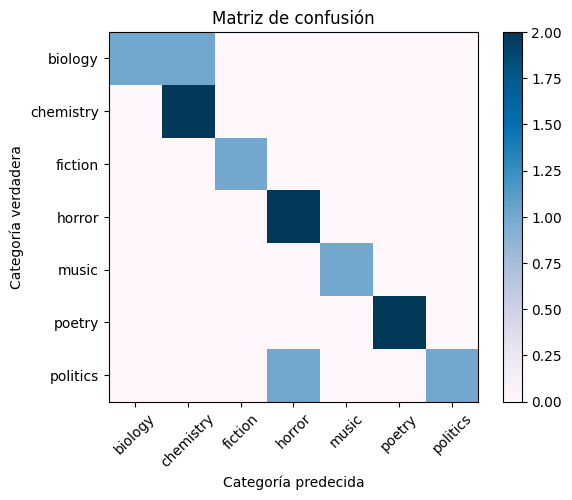
\includegraphics[scale=0.8]{../figures/confusion_matrix.png}
    \caption{Matriz de confusión.}
    \label{fig:confusion_matrix}
\end{figure}

Los resultados a las métricas TP, TN, FP, FN son las mostradas en la matriz de confusión, mientras que los resultados para el resto de las métricas pendientes son mostrados a continuación:
\begin{minted}[
frame=none,
autogobble,
obeytabs=false,
breaklines,
tabsize=4,
linenos=true,
baselinestretch=1,
firstnumber=1,
bgcolor=\bgrepl,
numberblanklines=false,
]{python}
# REPL

>>> print(classification_report(label_test, label_predicted, zero_division=0))

              precision    recall  f1-score   support
     biology       1.00      0.50      0.67         2
   chemistry       0.67      1.00      0.80         2
     fiction       1.00      1.00      1.00         1
      horror       0.67      1.00      0.80         2
       music       1.00      1.00      1.00         1
      poetry       1.00      1.00      1.00         2
    politics       1.00      0.50      0.67         2

    accuracy                           0.83        12
   macro avg       0.90      0.86      0.85        12
weighted avg       0.89      0.83      0.82        12
\end{minted}

De la matriz de confusión en la \cref{fig:confusion_matrix} se puede observar que hay dos libros que están mal clasificados. Esto sepuede verificar al observar la comparación en la tabla mostrada anteriormente donde se listaron las categorías reales y las predichas. Uno de lo libros en la categoría de biología fue mal clasiicado en la categoría de química, mientras que un libro de política se clasificó dentro de la categoría de horror.

Al inicio de este estudio se notó que la cantidad de libros requerida para este trabajo era poca, esto se vió reflejado en la pobre clasificación de los textos, y por ello se decidió incluir más categorías con más libros por categoría. El número de libros por categoría que se muestra al inicio del trabajo en el desglose dependió de en qué punto comenzaban a mejorar las predicciones. Se esperaba que con mayor diversidad de categorías, siendo éstas menos similares las unas con las otras, se obtuviera como resultado una mejor clasificación. 

Uno de los primeros intentos al escribir este trabajo se realizó incluyendo a la categoría de ficción y a la de horror, con política y cuentos infantiles, con 5 libros por categoría. Resultó en una pobre clasificación ya que los libros elejidos influían fuertemente en la clasificación. La ficción es un género literario bastante general, este género tiene muchos subgéneros. A pesar de no ser iguales, la ficción al horror, son similares, y eso hace que la elección de libros importe en este caso. Algo similar sucedió con los libros elegidos inicialmente para la categoría de cuentos infantiles.

Con los ajustes pertinentes, y una selección más detallada de los libros respecto a sus categorías, se logró que la mayoría de los libros en el conjunto de prueba fuesen clasificados correctamente. Una de las razones por las cuales uno de los libros en la categoría de biología fuese reconocido como perteneciente a la categoría de química es porque en ambas áreas de las ciencias suelen tener vocabulario técnico y no técnico similar ya que están fuertemente relacionadas.

% \begin{minted}[
%     frame=none,
%     autogobble,
%     obeytabs=false,
%     breaklines,
%     tabsize=4,
%     linenos=true,
%     % numbersep=-10pt,
%     baselinestretch=1,
%     firstnumber=last,
%     bgcolor=bg!70,
%     ]{julia}
% \end{minted}

% \clearpage
% \section*{Apéndice}
% \inputminted[
%     frame=none,
%     autogobble,
%     obeytabs=false,
%     breaklines,
%     tabsize=4,
%     linenos=true,
%     % numbersep=-10pt,
%     baselinestretch=1,
%     firstnumber=1,
%     bgcolor=bg!70,]{julia}{\codepath}

\nocite{*} % to call all references even if they are not cited in the text
\bibliography{references.bib}

\end{document}